%%%%%%%%%%%%%%%%%%%%%%%%%%%%%%%%%%%%%%%%%%%%%%%%%%%%%%%%%%%
% Appendix file
% Goal: provide appendix for my MSc thesis
% Authors: Gaiëtan Renault <gaietan.renault@alumni.epfl.ch>
%
% This work may be distributed and/or modified under the
% conditions of the LaTeX Project Public License, either version 1.3
% of this license or (at your option) any later version.
% The latest version of this license is in
%   http://www.latex-project.org/lppl.txt
%
%%%%%%%%%%%%%%%%%%%%%%%%%%%%%%%%%%%%%%%%%%%%%%%%%%%%%%%%%%%

\appendix
\appendixpage
\addappheadtotoc

% %%%%%%%%%%%%%%%%%%%%%%%%%%%%%%%%%%%%%%
\chapter{Graphical Realism Framework for Industrial Control Simulation}
%\begin{sidewaysfigure}
\label{ch:GRFICS}

\begin{figure}[H]
    \centering
    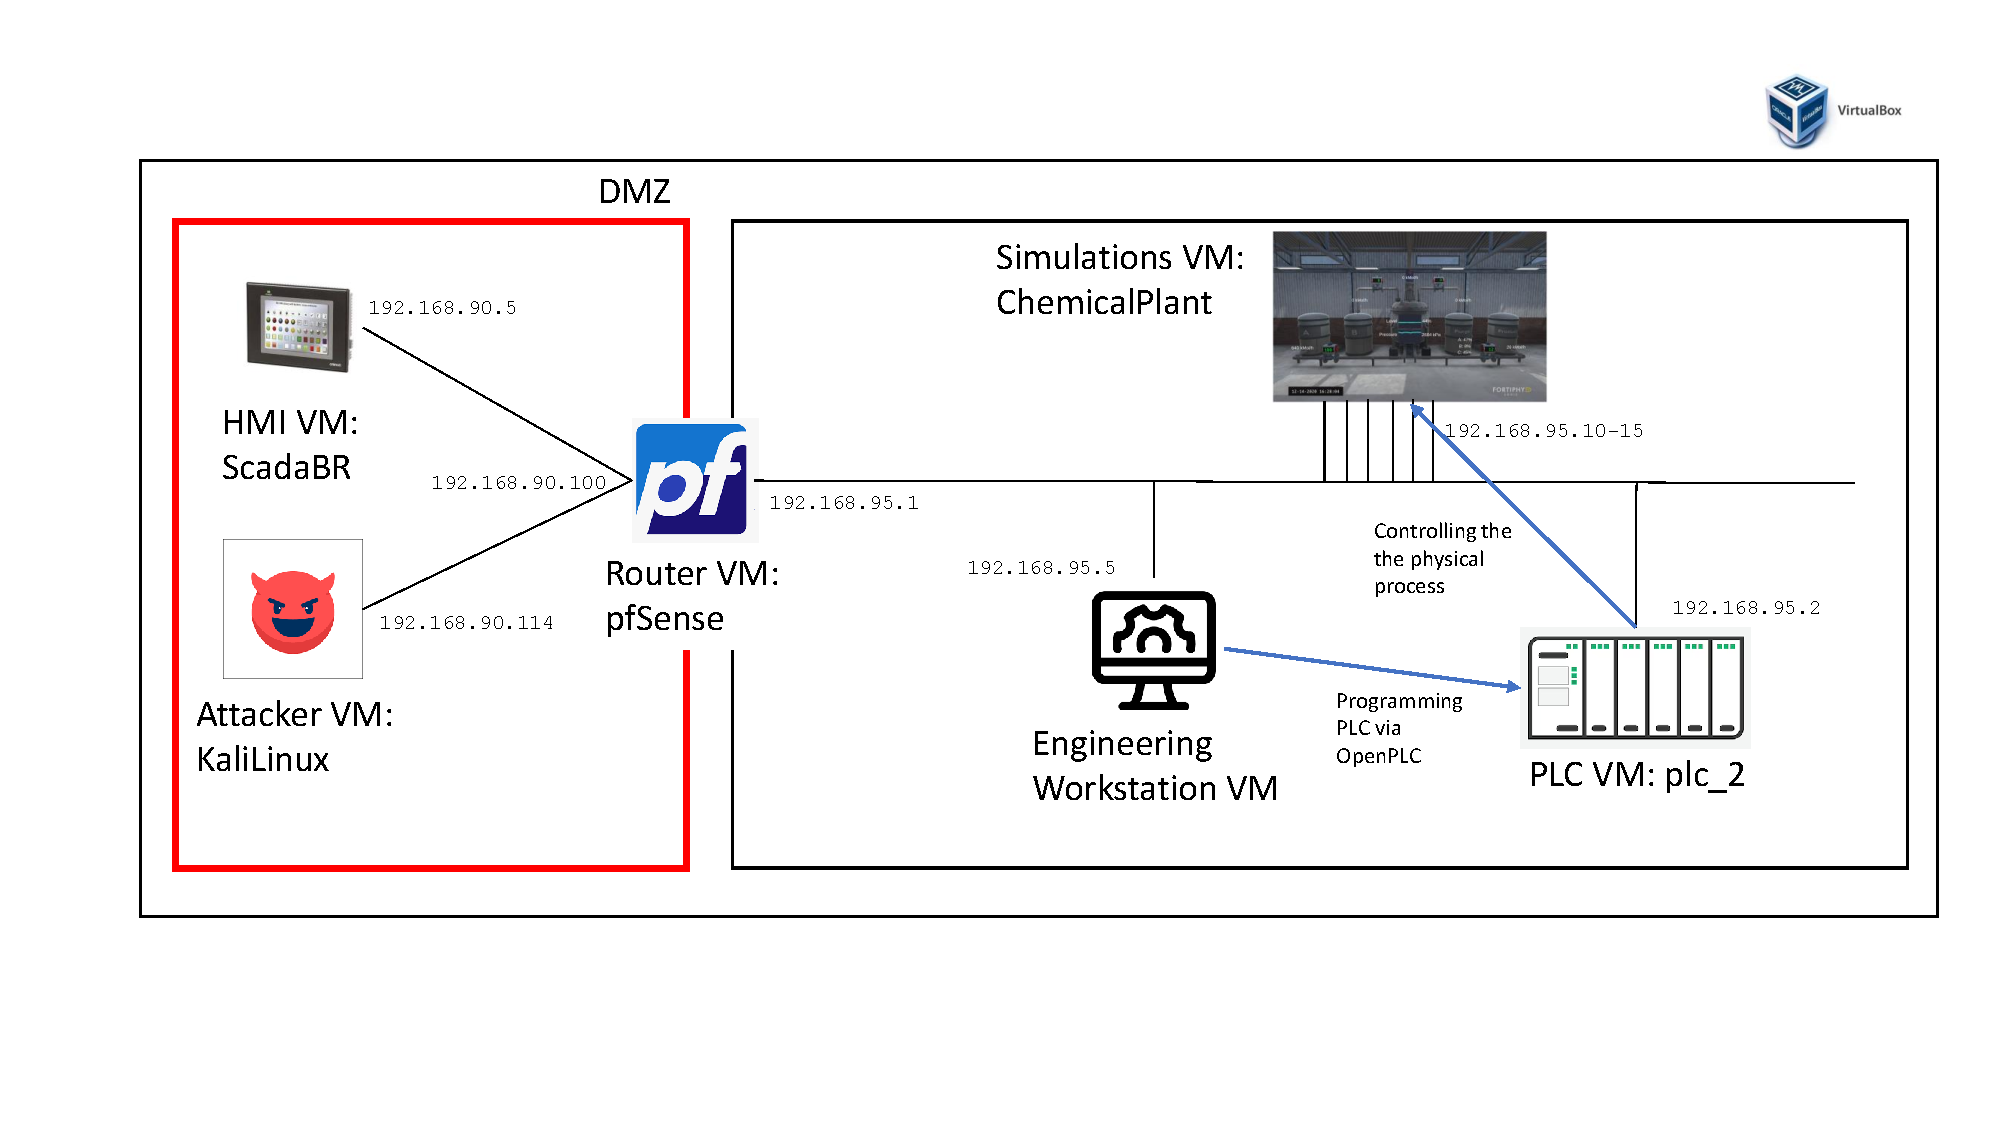
\includegraphics[width=\linewidth, trim={1cm 3cm 1cm 1cm}, clip]{figures/GRFICSv2_net_arch.pdf}
    \caption{Network architecture of the GRFICSv2. The GRFICSv2 makes use of six VMs (e.g, attacker, HMI, firewall, Engineering Workstation, PLC, and 3D process simulation) to model a cyberattack leading to an explosion of a chemical process.}
    \label{fig:GRFICSv2_arch}
\end{figure}

\chapter{Pressurized Water Reactor (PWR)}
\label{ch:pwr}
\begin{figure}[H]
    \centering
    \vspace{-1cm}
    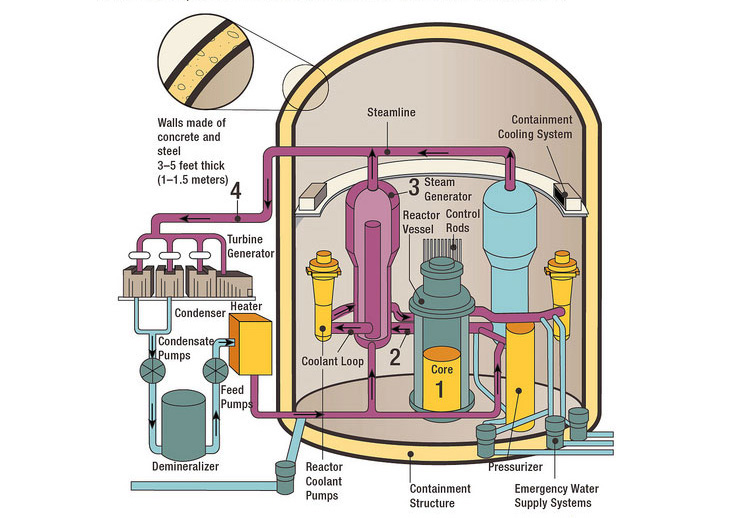
\includegraphics[width=\linewidth]{figures/pwr.jpg}
    \caption{Pressurized Water Reactor \cite{imgPwr}. 1. The core, situated in the reactor vessel, produces heat from nuclear reaction. 2. Pressurized water in the primary circuit carries the heat to the steam generator. 3. Inside the steam generator, heat from the primary circuit vaporizes the water in a secondary circuit, producing steam. The steam then rotates the rotor of the turbine generator, producing electromagnetic field variation which induces alternating current in the stator.}
    \label{fig:pwr}
    \hfill
\end{figure}
 
\chapter{Reactor Containment Building (CB)}
\label{ch:reactor_building}
\begin{figure}[H]
    \centering
    \vspace{-1cm}
    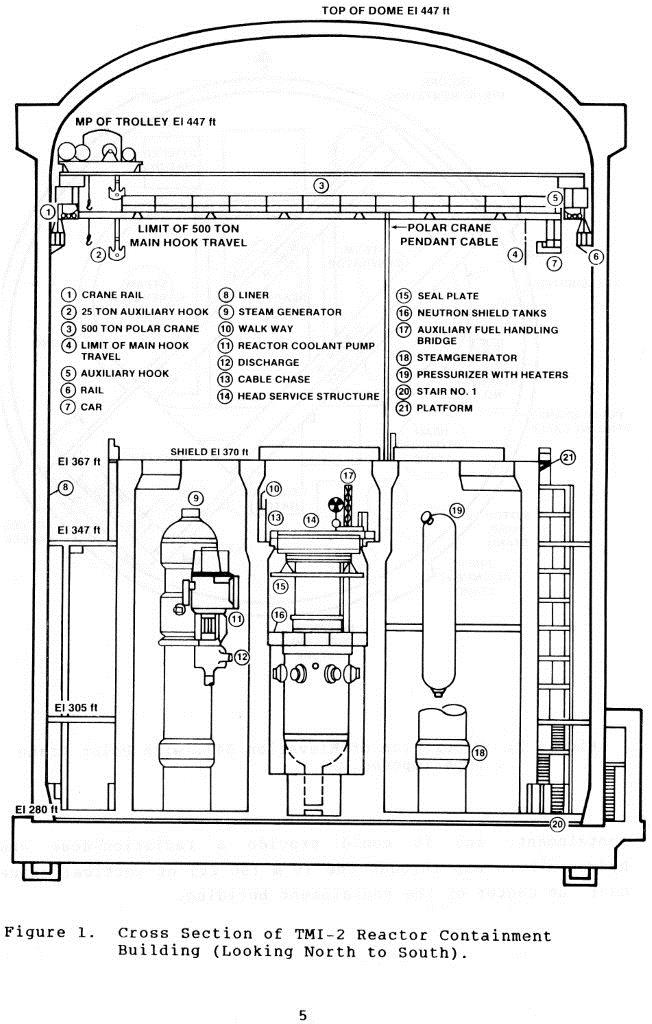
\includegraphics[width=0.5\linewidth]{figures/reactor_building.jpg}
    \caption{Reactor Containment Building (CB)~\cite{ONR-cs-br}. The Three Mile Island NPP CB is a 140 meters high and 80 cm thickness building that resists to internal accident situations (e.g., break of the primary circuit) and external aggressions (e.g., human origin or natural hazard).}
    \label{fig:reactor_building}
\end{figure}

\chapter{Purdue Model}
\begin{figure}[H]
    \centering
    \vspace{-0.75cm}
    \includegraphics[height=9cm]{figures/ICS-Purdue-Model.pdf}
    \caption{The Purdue Model: a Simplified Architecture of an ICS~\cite{imgPurdueModel}. The different levels an ICS architecture from Top to Bottom. 1. Level 5, in red, is the Corporate Network. This delocalized area is for example made of servers, or employees computer. 2. Level 4, in orange, is the Plant Network. It is mainly used for process reporting. 3. Level 3, in yellow, is the site control operations. It is separated with Level 4 by a DMZ that globally acts as a one-way firewall. The Level 3 is an area made for example of historians and process maintenance servers. The Level 2, in purple, is the SCADA. It is made of HMIs and allows technicians to visualize and supervise the process. The Level 1, in cyan, is the area process control it is mainly made of DCS (e.g., PLC, RTU or IIoT devices). The Level 0 is the process instrumentation made of actuators and sensors. As a side note, a polar crane's ICS is generally smaller and is an air-gap not connected to the Level 3 to 5.}
    \label{fig:purdue-model}
\end{figure}

\chapter{Threat Model}
\label{ch:threat_model}
\begin{figure}[H]
    \centering
    \vspace{-1.5cm}
    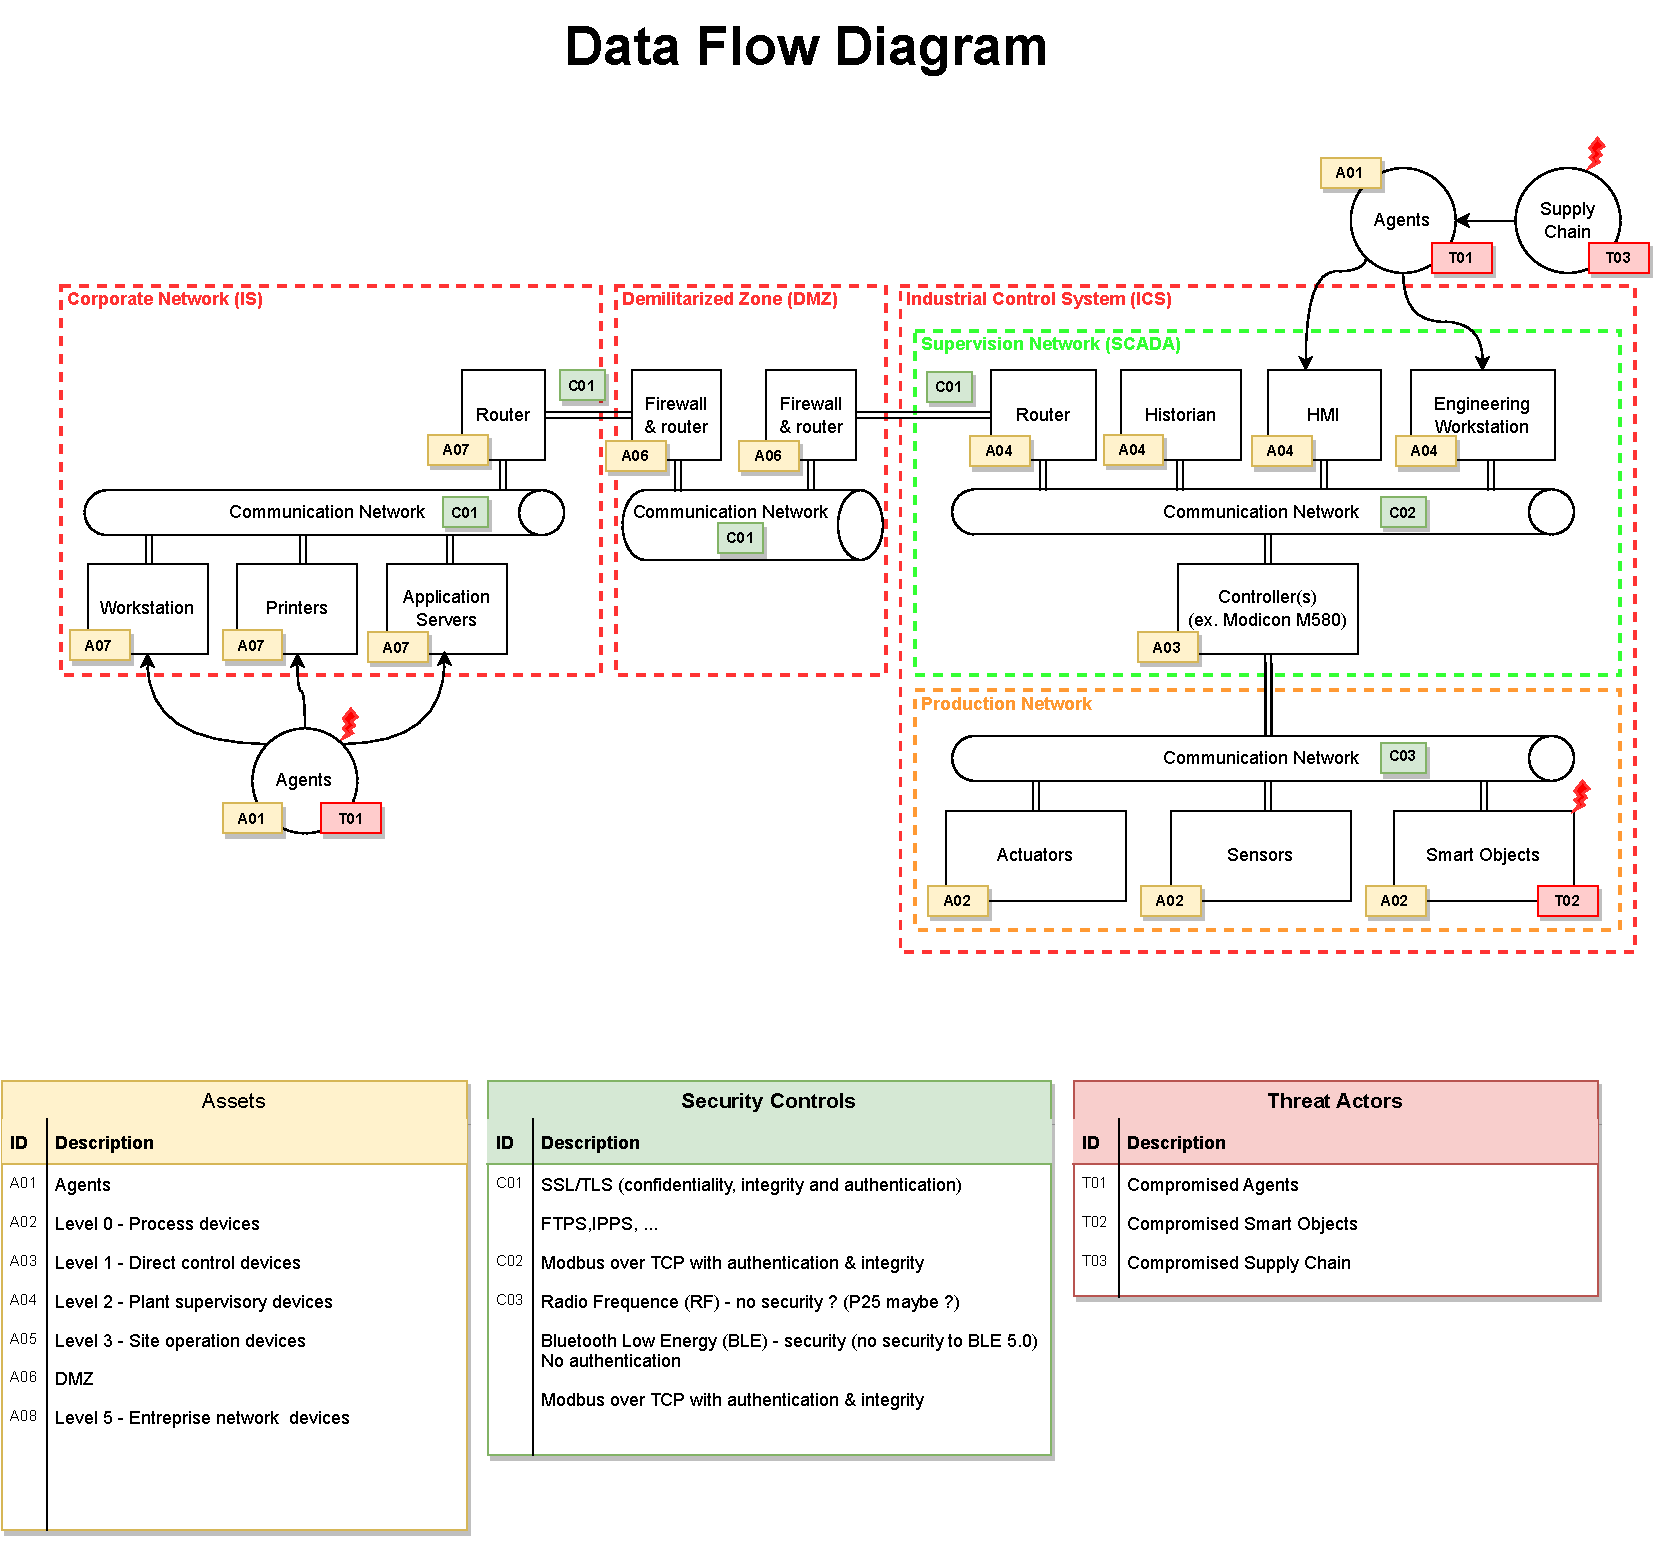
\includegraphics[height=12.7cm, angle=00, trim={0cm 0cm 0cm 2cm},clip]{figures/Threat-modelling-DFD.pdf}
    \caption{Data flow diagram. From an ICS architecture, this data flow diagram represents the three entry points identified – the corporate network, the supervision network, or the production network. The \emph{NinjaCrane} attack infects first the supervision network via a malicious HID USB to then tamper the production network.}
    \label{fig:data_flow_diagram}
\end{figure}

\begin{figure}
    \centering
    \vspace{2cm}
    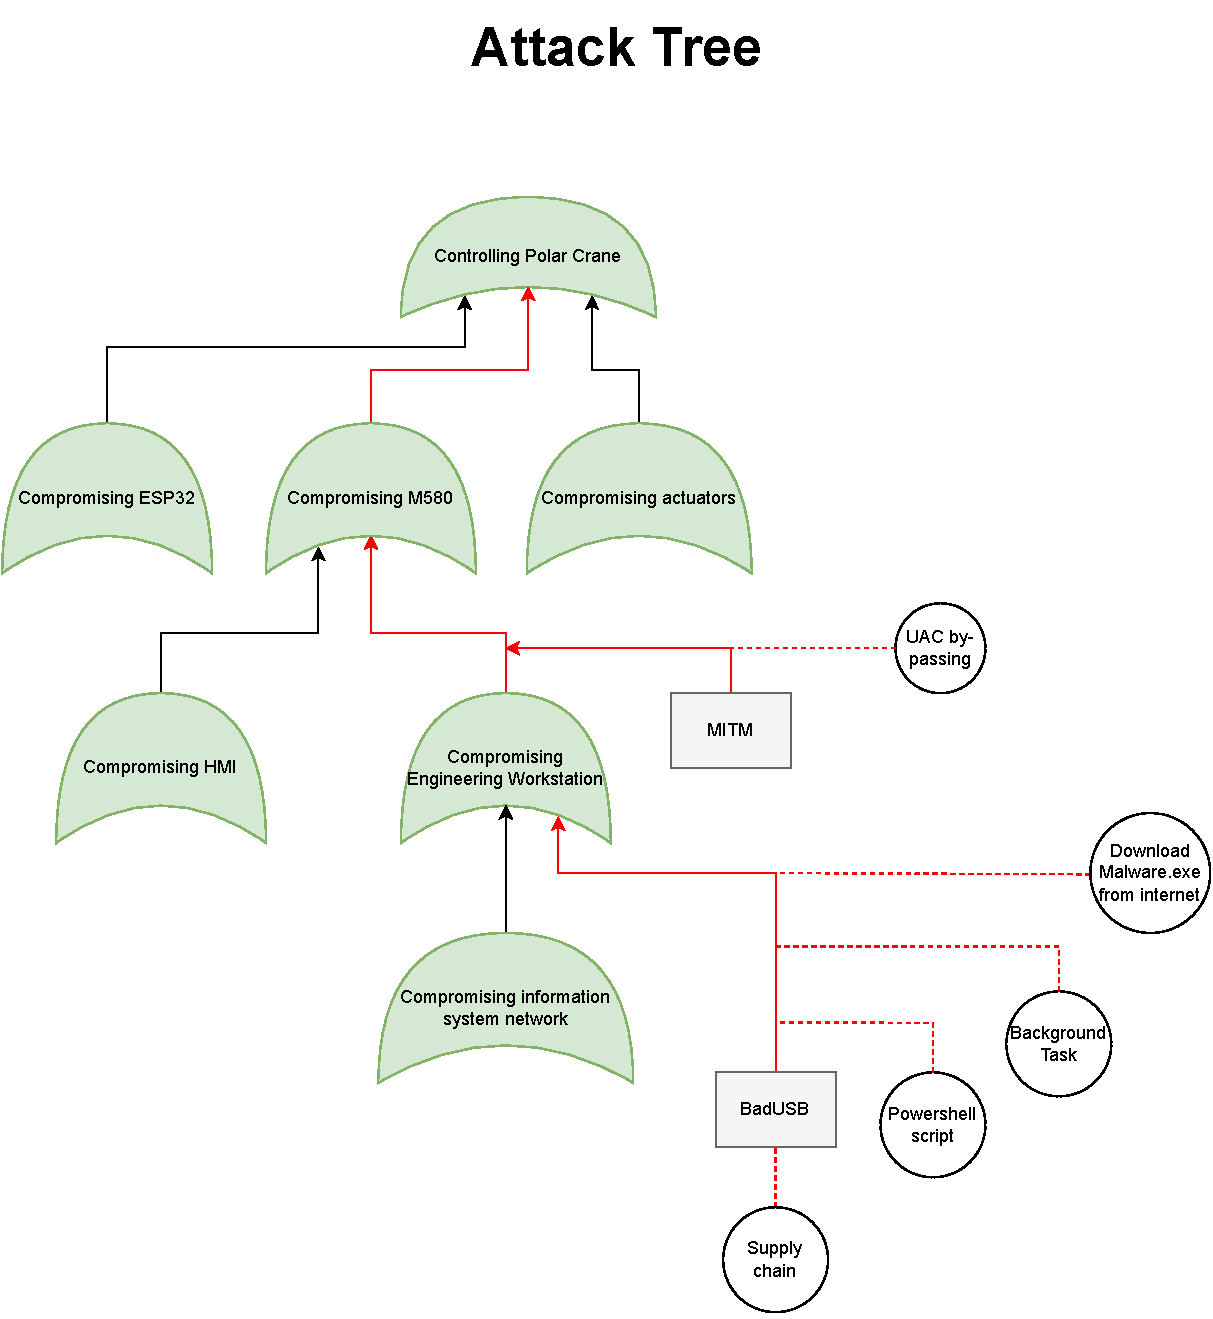
\includegraphics[height=12cm, angle=90, trim={0cm 0cm 0cm 2cm},clip]{figures/Threat-modelling-Attack Tree.pdf}
    \caption{Attack tree. The attack tree models the path taken to take control over the polar crane. The first step is the supply chain compromising that brings a HID-capable device to be connected to the engineering workstation. When connected, the USB device runs a powershell script to download and execute in background a malware. This malware by-pass the windows UAC and performs a MITM attack to modify PLC's internal variables and take control over the polar crane.}
    \label{fig:atk-tree}
\end{figure}

\chapter{Polar Crane's Testbed}

\begin{figure}[H]
    \centering
    \vspace{-1.3cm}
    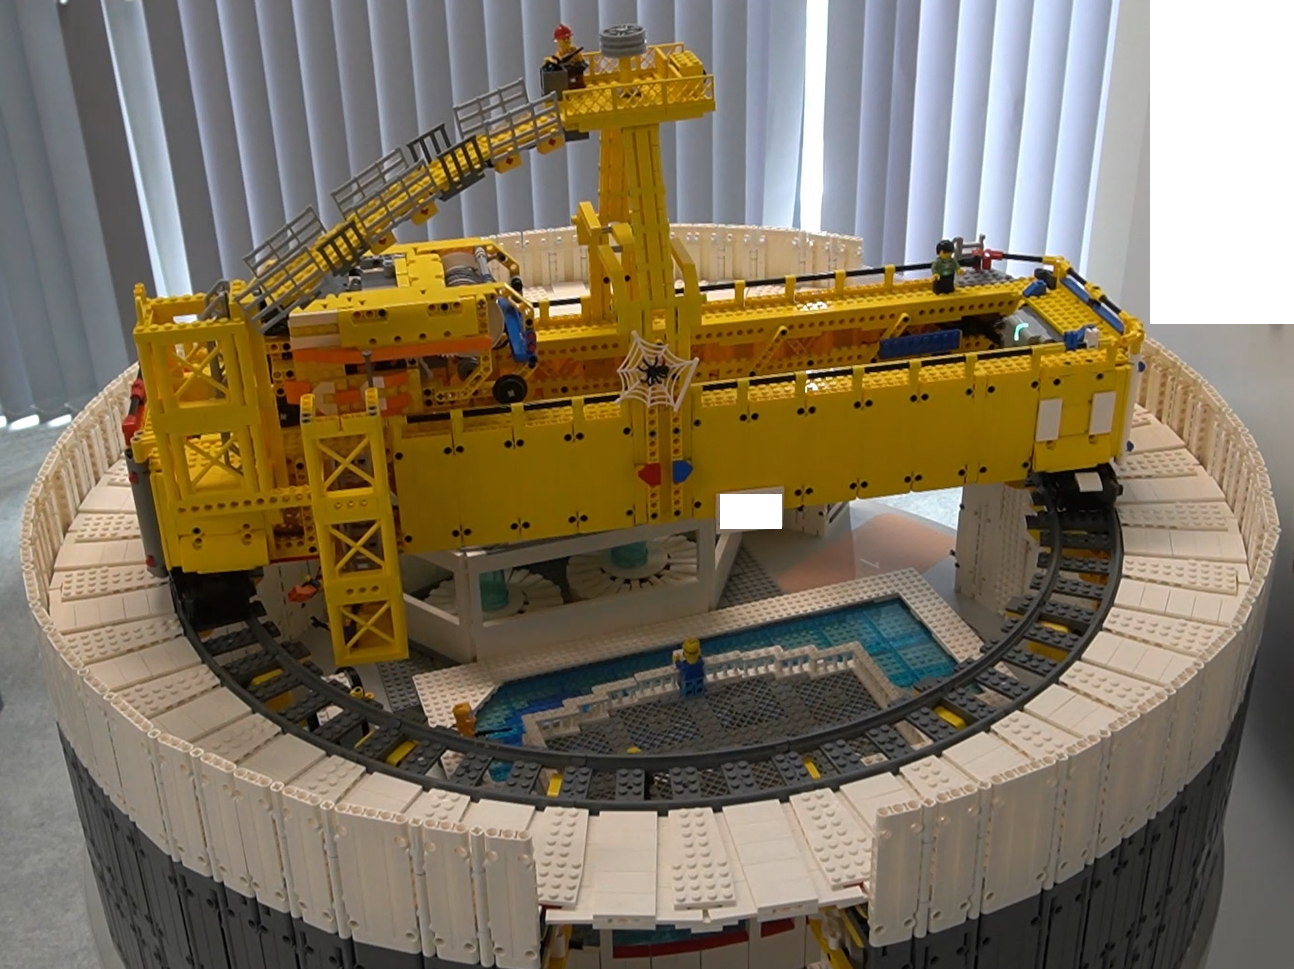
\includegraphics[width=\linewidth]{figures/polar-crane}
    \caption{Polar Crane's Sketch. Sketch in LEGO\texttrademark of the polar crane which models three different movements; crane rotation, trolley rectilinear displacement, and charge lift. Those movements are controlled via an HMI connected to the \emph{Modicon M580} PLC. The PLC interprets and transmits the commands to three LEGO\texttrademark BLE Hubs via an ESP32 microcontroller establishing the Bluetooth connection.}
    \label{fig:polar-crane}
\end{figure}

\begin{figure}
    \centering
    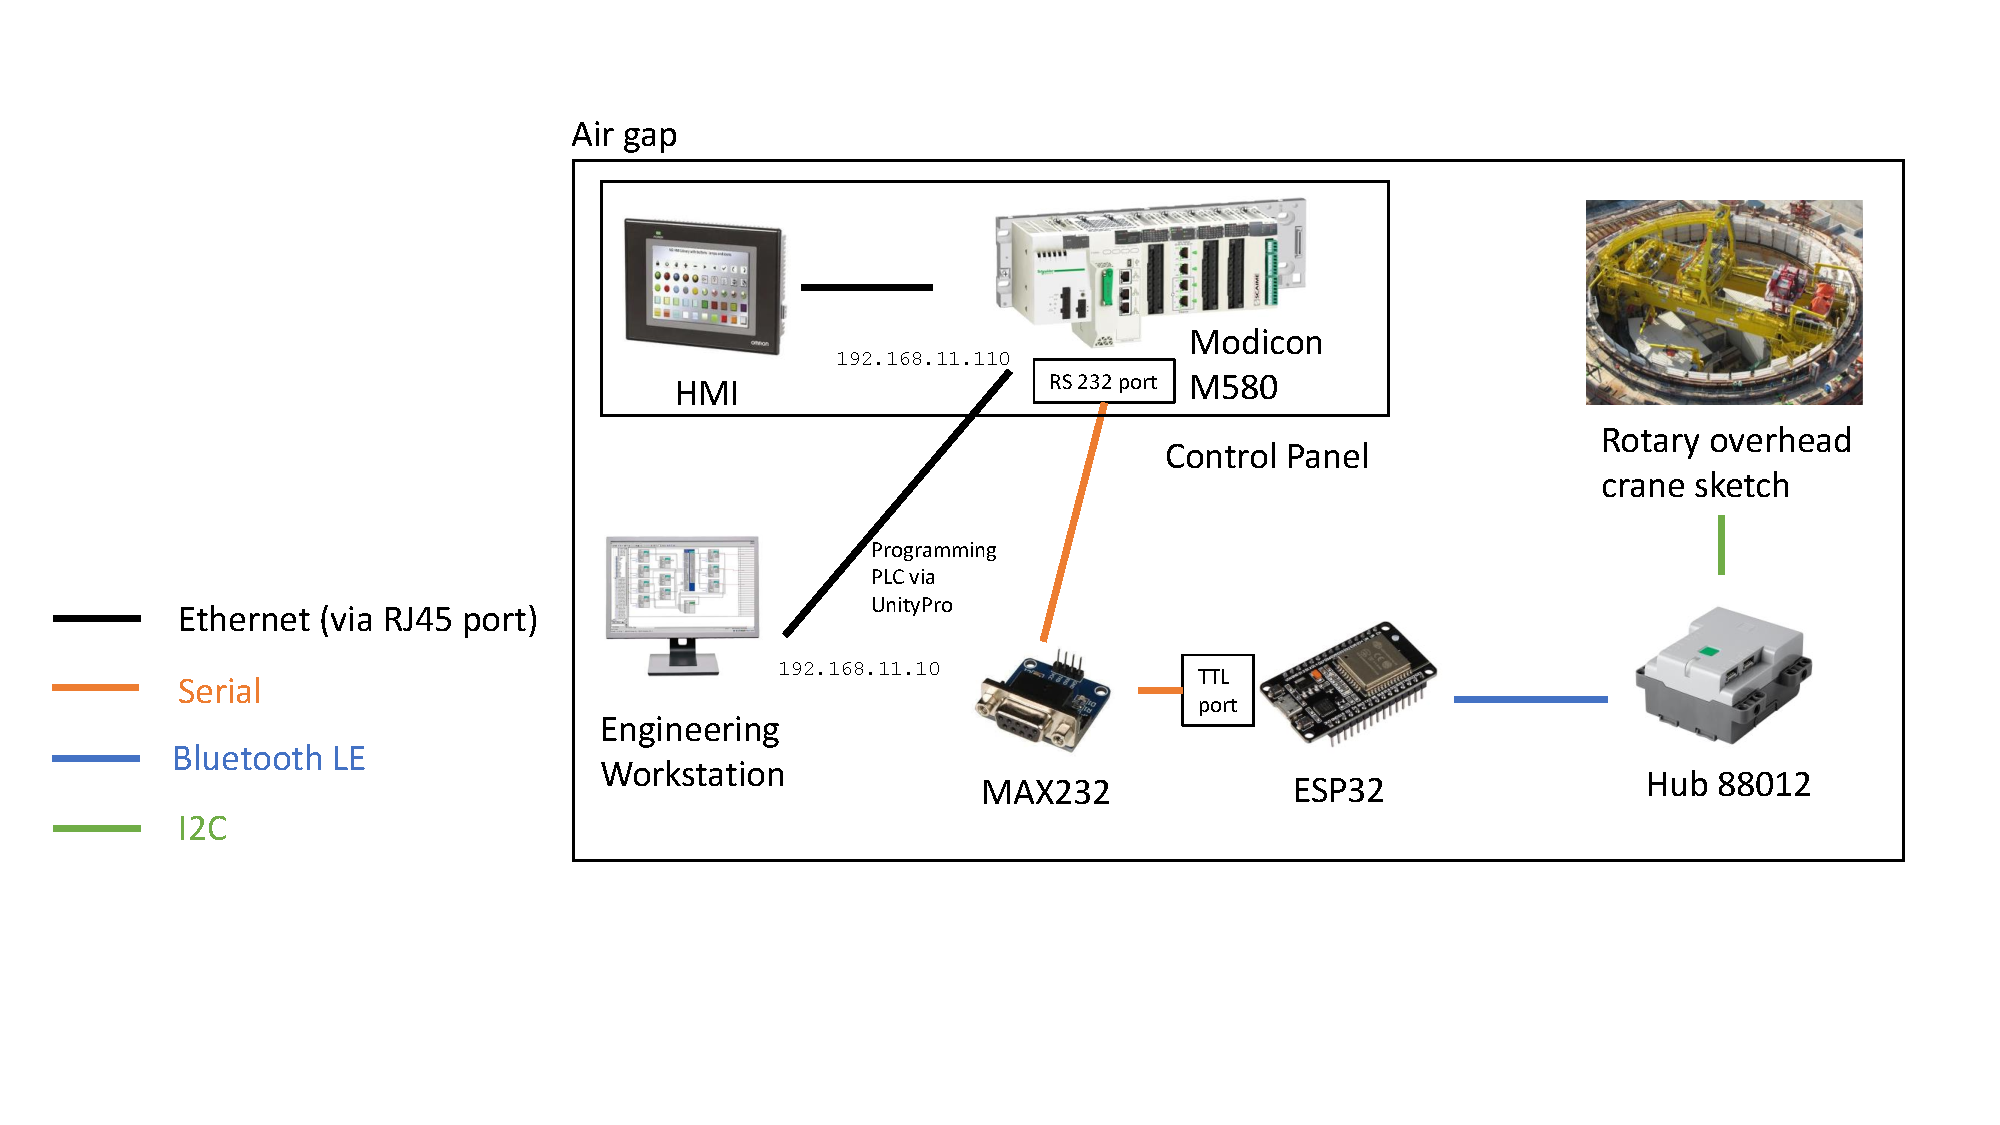
\includegraphics[width=\linewidth]{figures/Setup.pdf}
    \caption{Network Architecture of the Testbed. The Engineering Workstation programs the M580 PLC via Unity Pro. The M580 stores and executes the polar crane's program. The HMI displays the state (i.e., position, speed etc.) of the polar crane and allows a technician operator to control the polar crane. Due to its rotation, the polar crane must be controlled over the air. In this testbed the choice has been made to control the polar crane with BLE. The ESP32 is sending over BLE the commands it received from the PLC.}
    \label{fig:setup}
\end{figure}

\chapter{Malicious Mouse}
\begin{figure}[H]
    \centering
    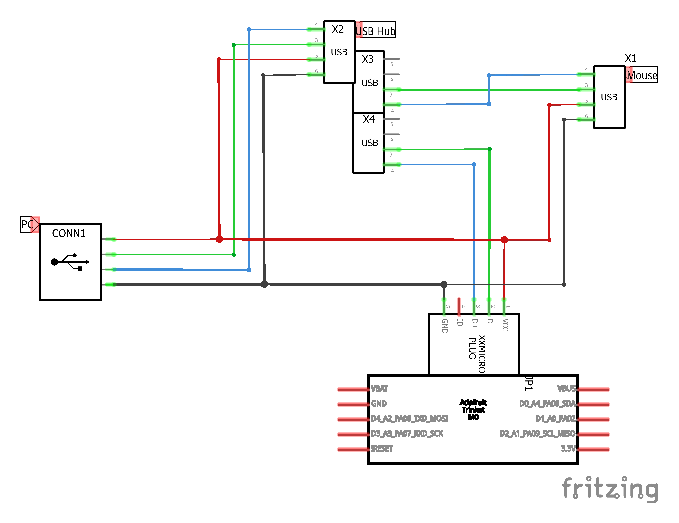
\includegraphics[height=9cm, angle=90, trim={0cm 0cm 0cm 0cm},clip]{figures/Sketch_wired_mouse_basUSB.pdf}
    \caption{Electric wired schematic of the malicious mouse. The mouse connection originates from the  \texttt{CONN1} (e.g., PC USB connection) and proceeds to an USB hub that splits the connection into two pathways – one leading to the mouse itself and the other one to an HID-capable microcontroller.}
    \label{fig:infected-mouse-wiring}
\end{figure}

\begin{figure}
    \centering
    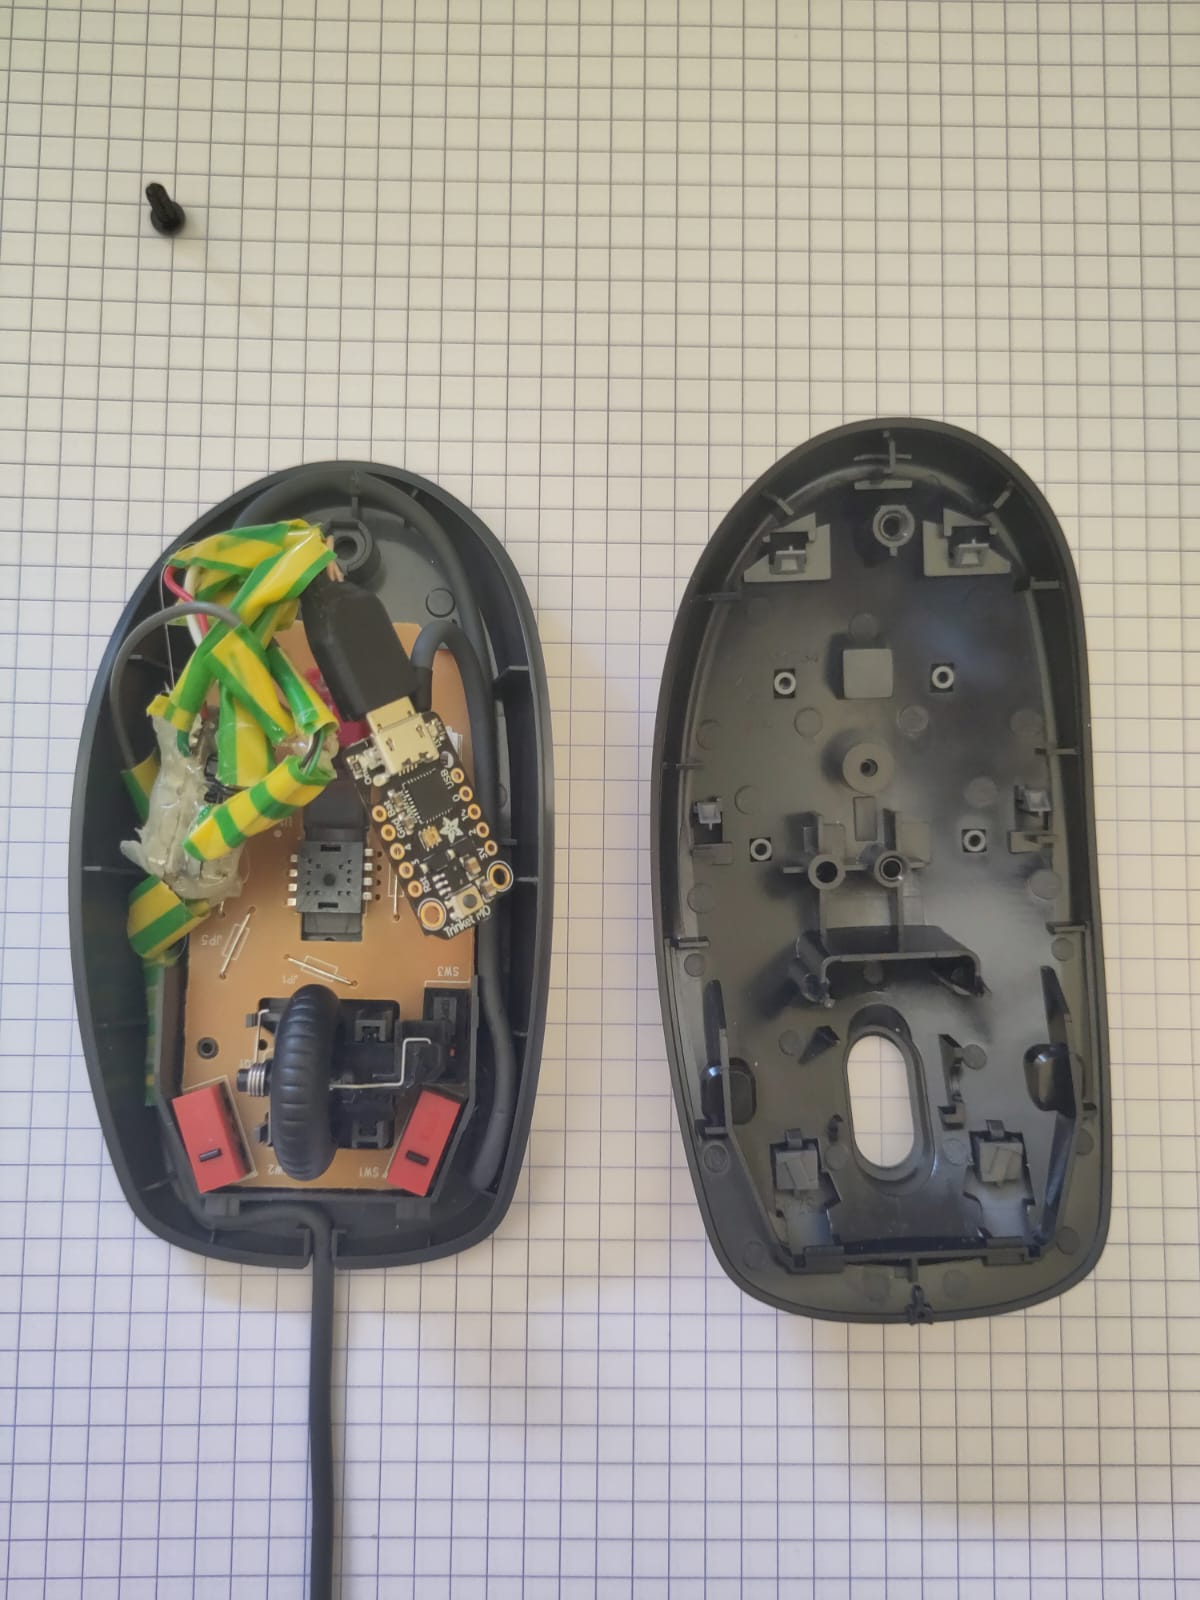
\includegraphics[height=13cm, trim={0cm 5cm 0cm 5cm},clip]{figures/infected-mouse.jpeg}
    \caption{Picture of the maliciously modified mouse. A Logitech mouse opened and modified in order to include an HID-capable microcontroller. On the photograph can be seen the Adafruit Trinket M0 connected in micro-USB to the hub.}
    \label{fig:infected-mouse-photo}
\end{figure}

\chapter{Modbus/UMAS Communication}
\begin{figure}[H]
    \centering
    \vspace{-0.5cm}
    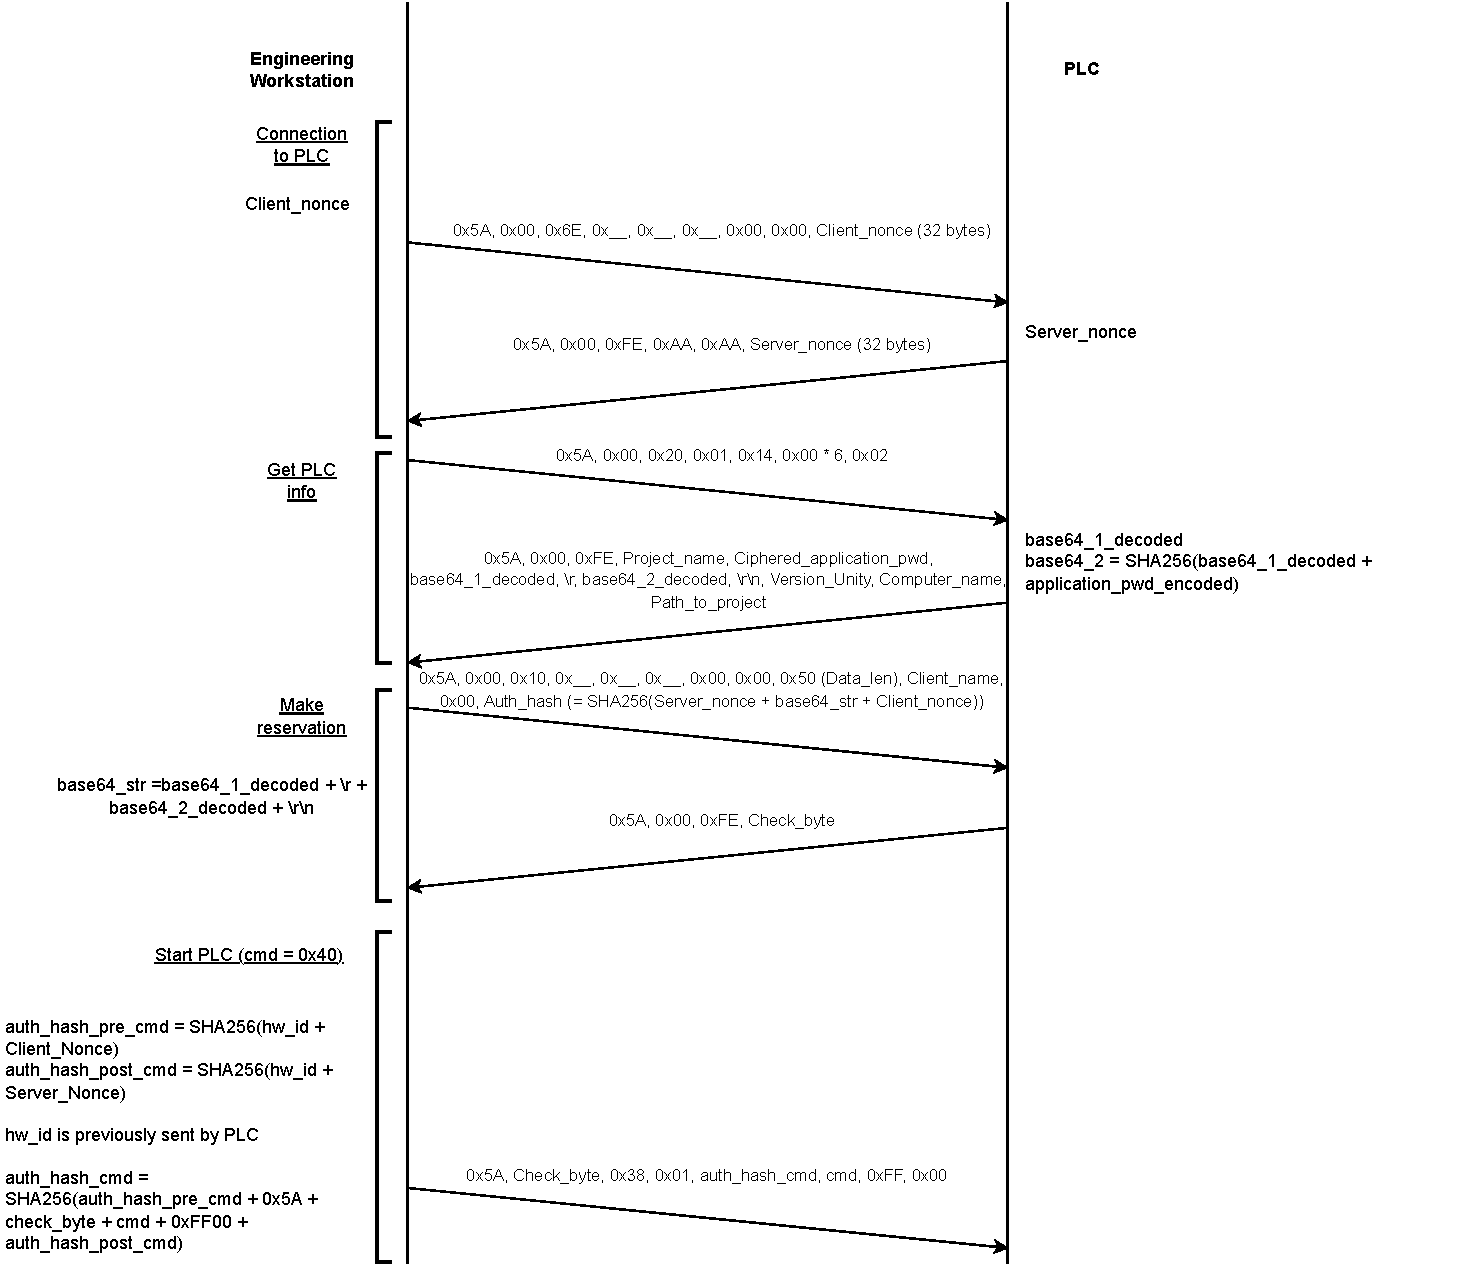
\includegraphics[width=0.95\linewidth]{figures/ModiPwn-Page-1.pdf}
    \caption{Communication between the M580 and the engineering workstation}
    \label{fig:communication}
\end{figure}

\chapter{Adversary's Graphical User Interface (GUI)}
\begin{figure}[H]
    \centering
    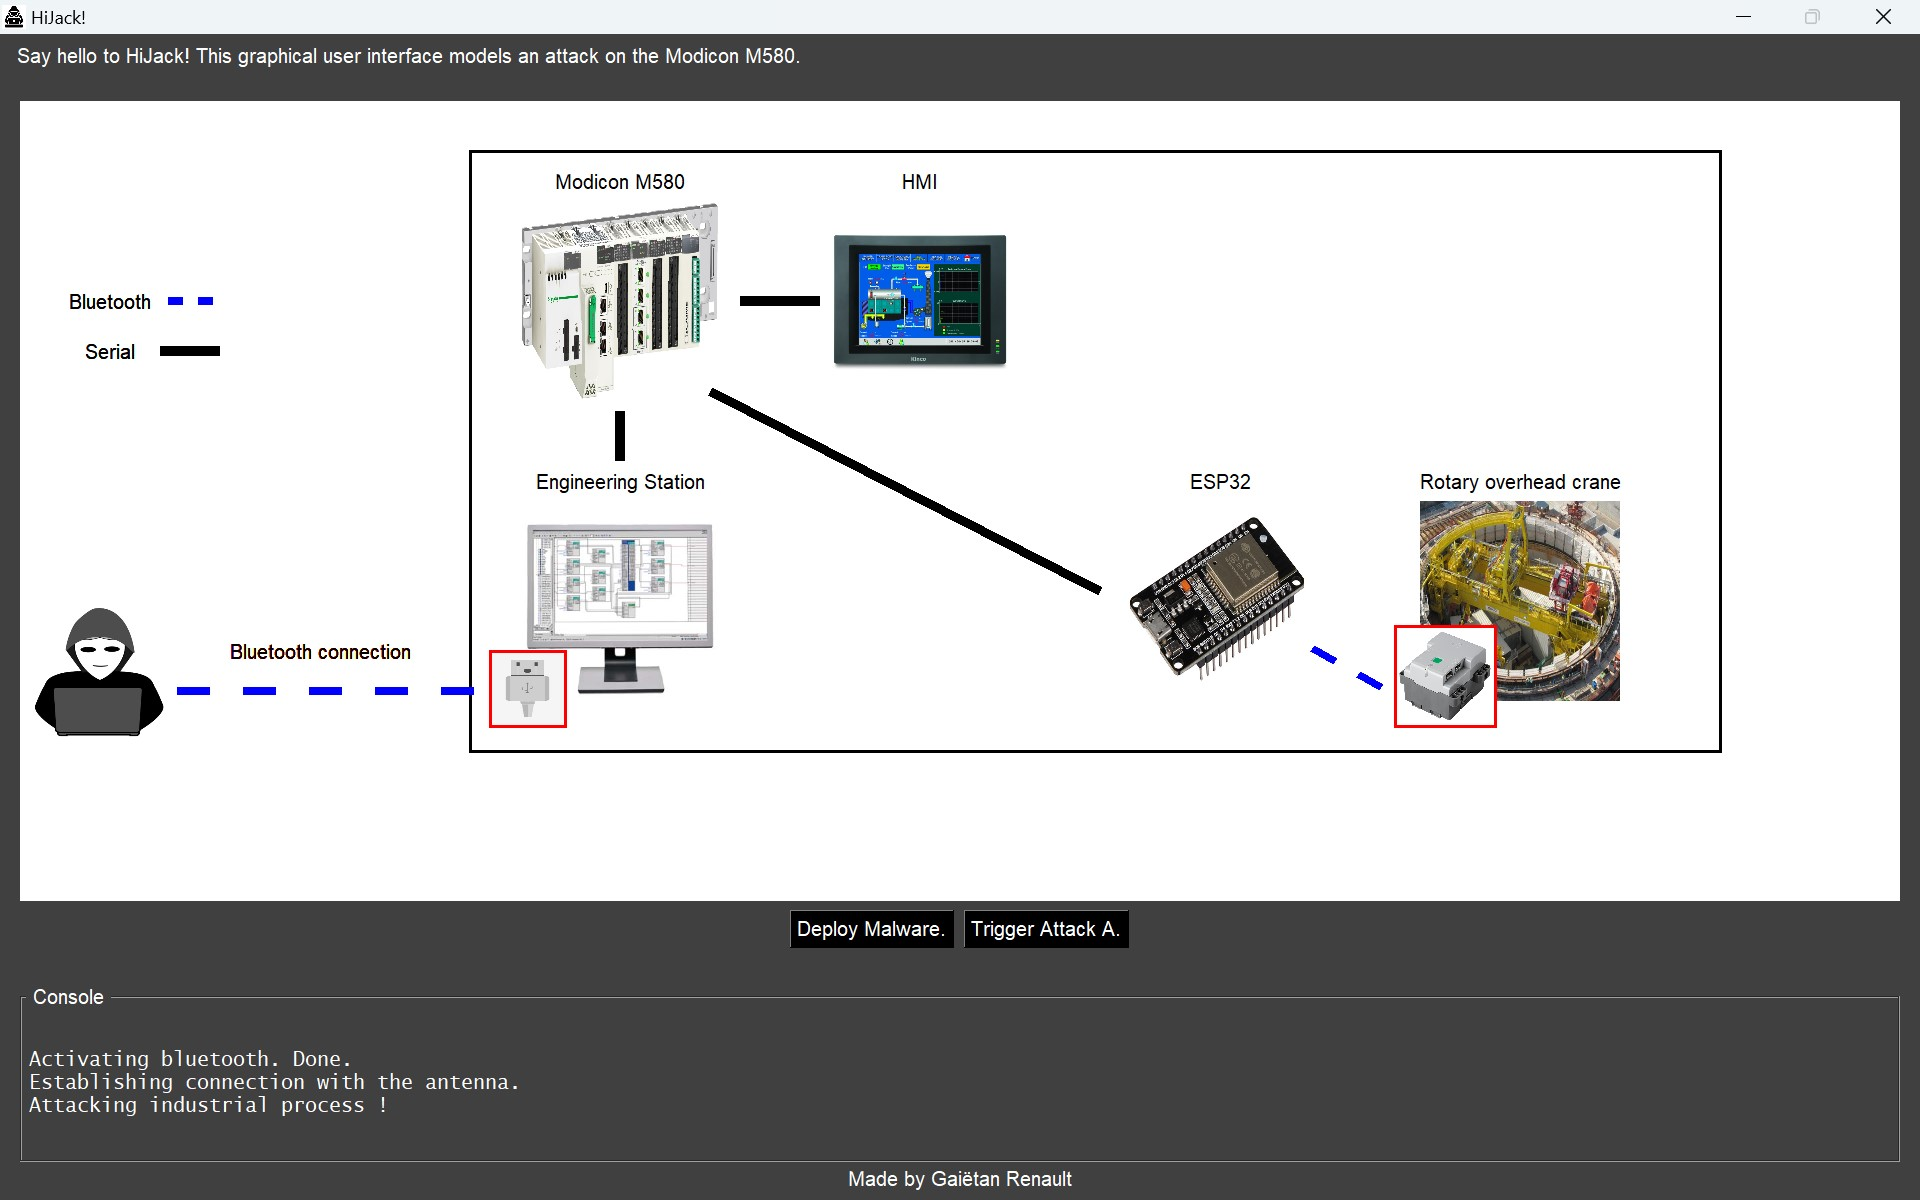
\includegraphics[width=\linewidth, angle=00, trim={0cm 0cm 0cm 0cm},clip]{figures/GUI.jpg}
    \caption{Adversary's Graphical User Interface (GUI). This interface, running on a laptop, is made with \href{https://www.pysimplegui.org/en/latest/}{\emph{PySimpleGUI}} and allows to take control of the USB Ninja cable over BLE by triggering two different payloads. The first one deploys the malware on the PC, the second one starts the \emph{NinjaCrane} attack.}
    \label{fig:gui}
\end{figure}

\chapter{Data Exfiltration}
\begin{figure}[H]
    \centering
    \vspace{-0.5cm}
    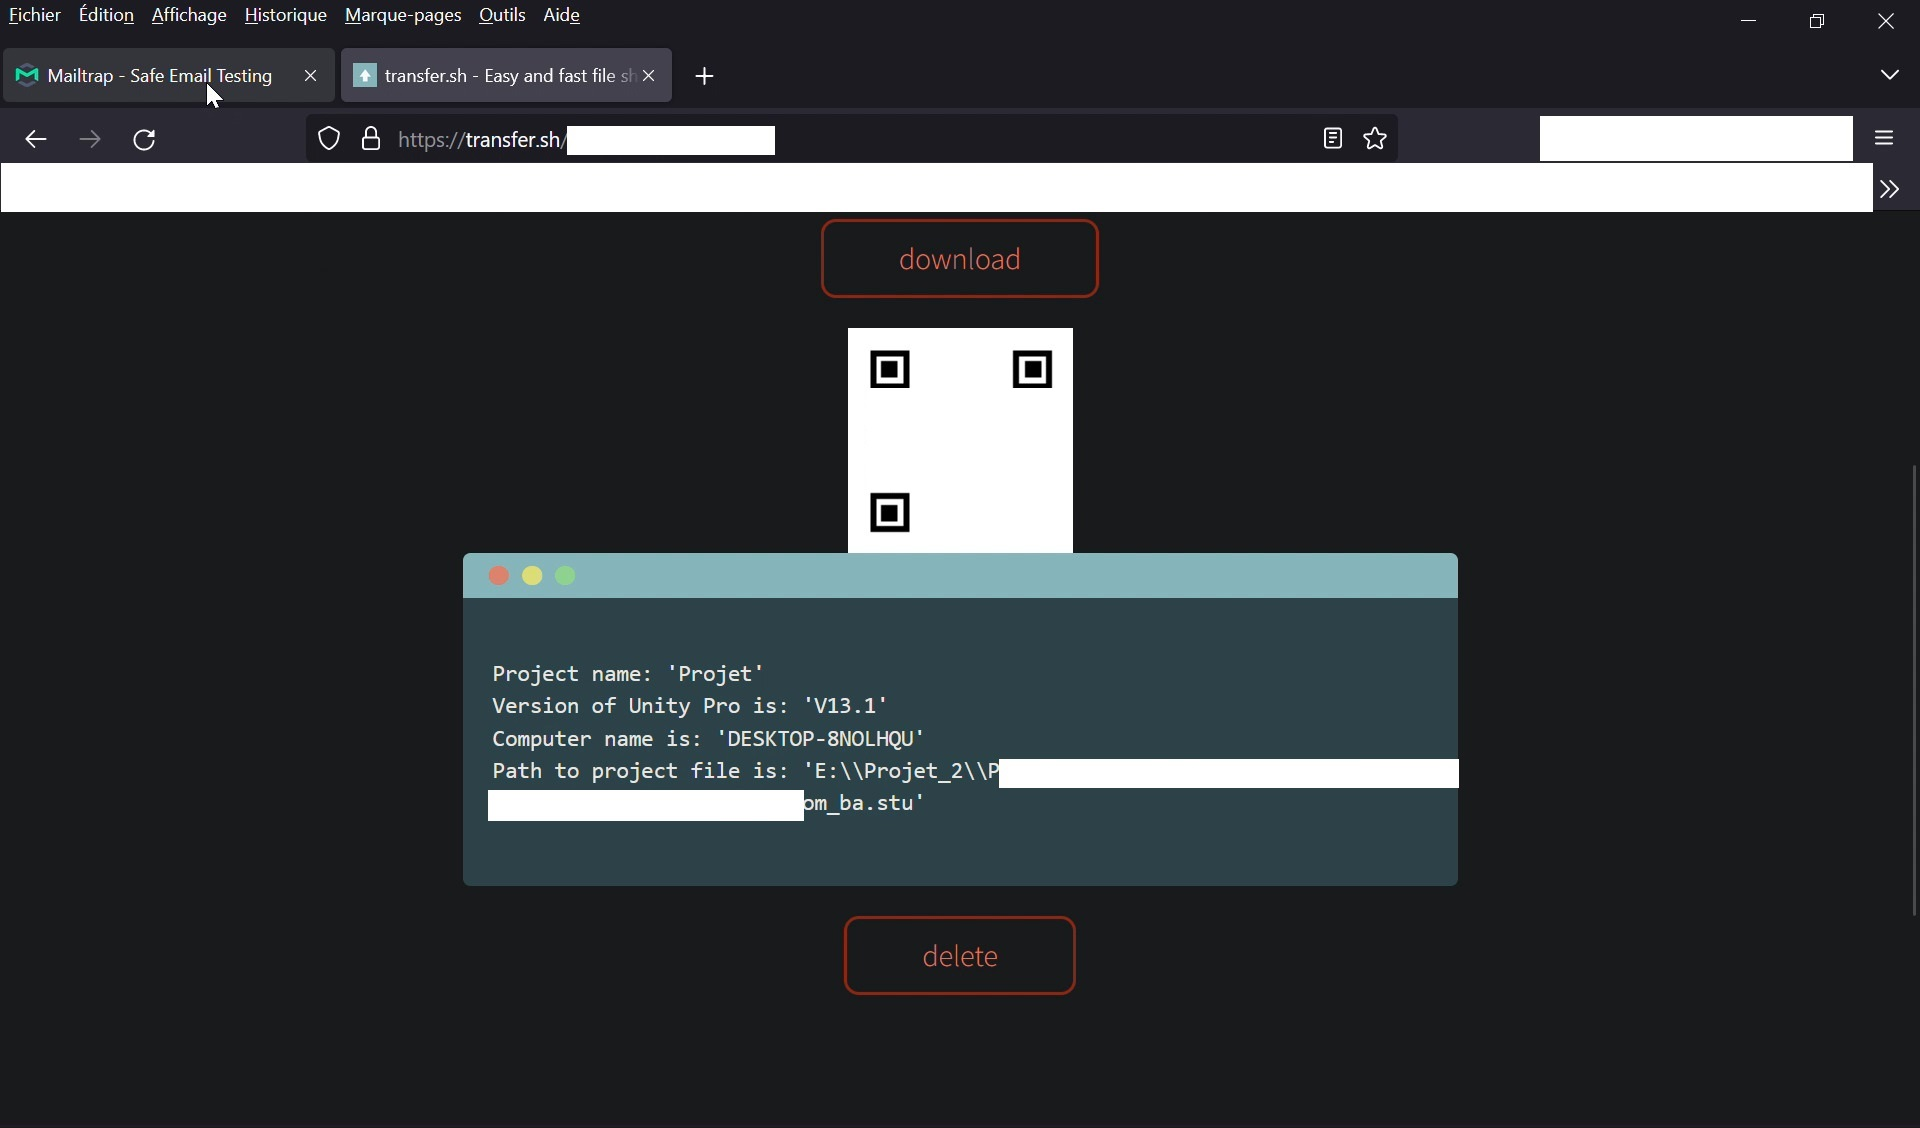
\includegraphics[width=0.7\linewidth]{figures/mailtrap-project-infos.jpg}
    \\ \vspace{0.5cm}
    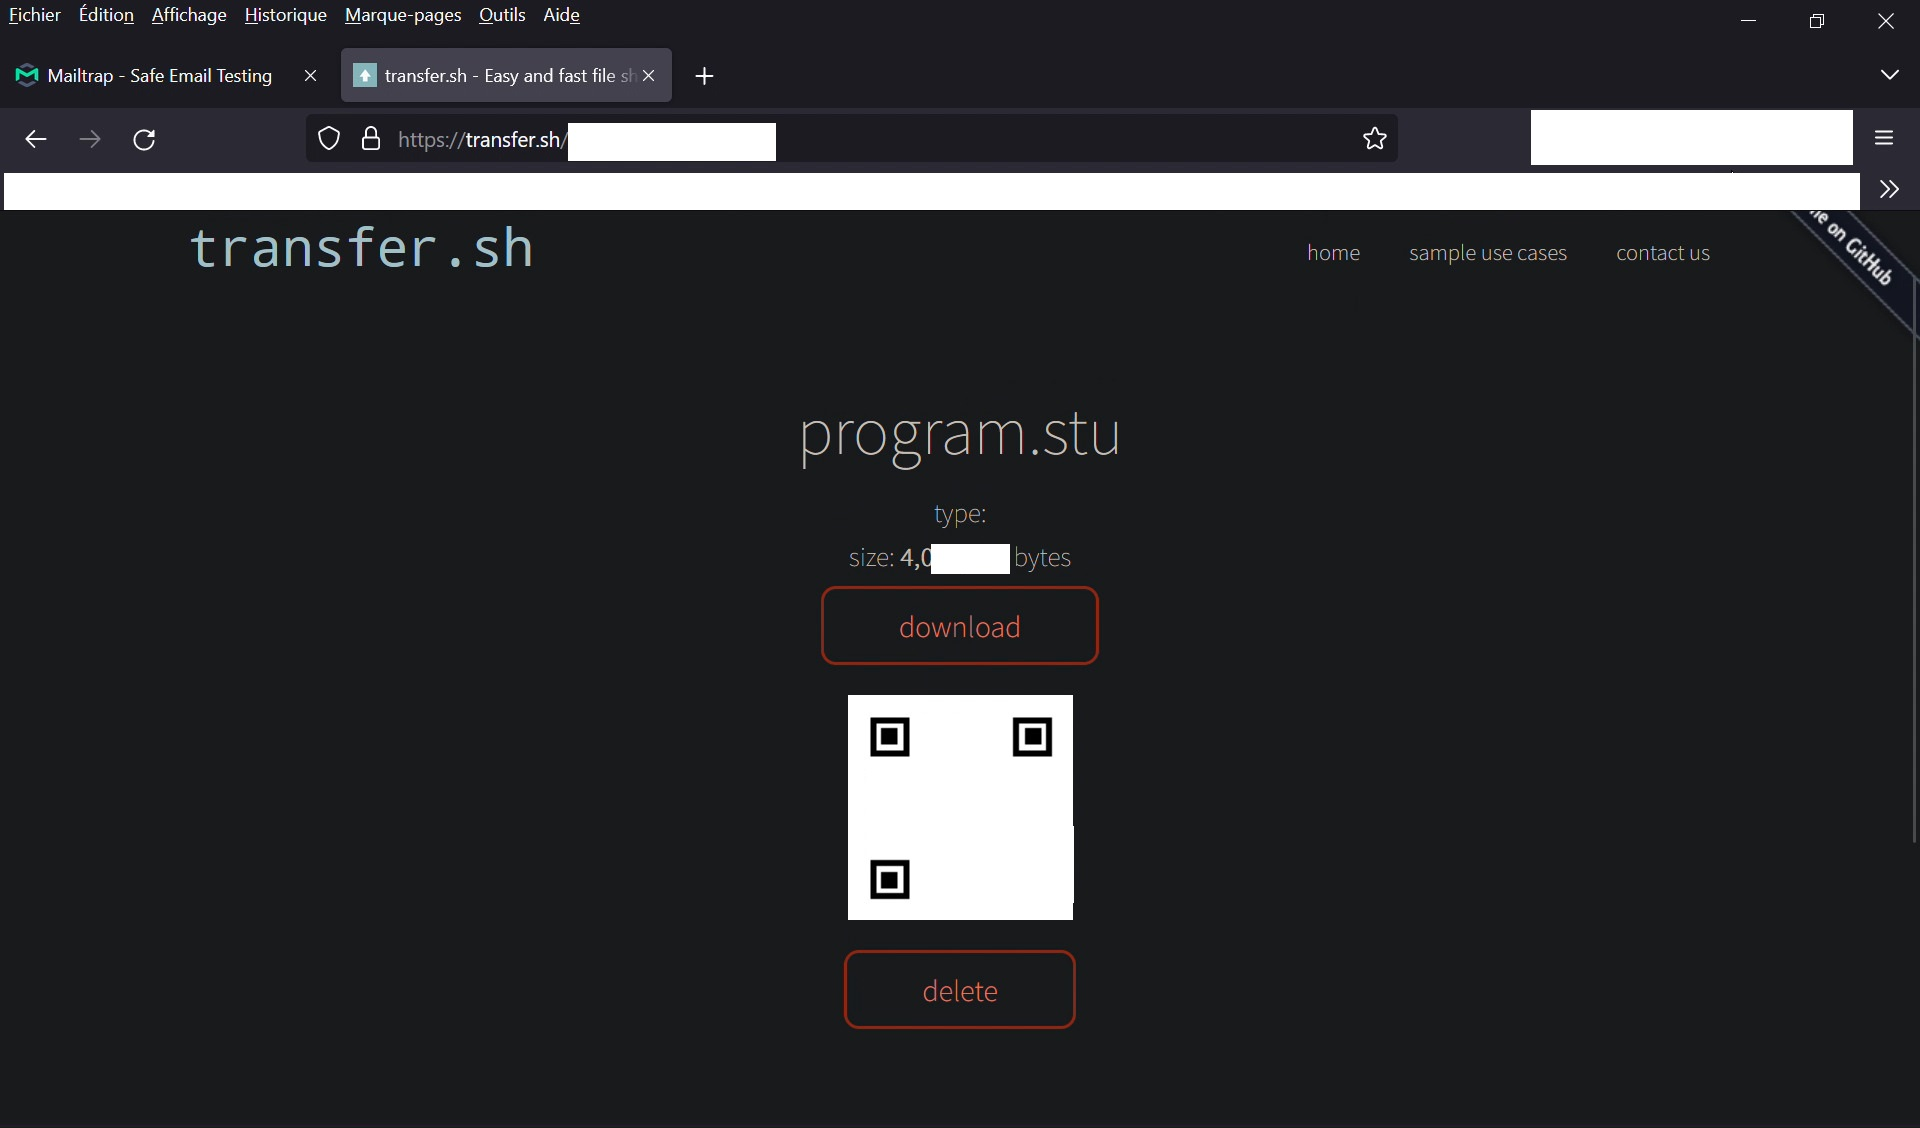
\includegraphics[width=0.7\linewidth]{figures/mailtrap-stu.jpg}
    \caption{Data exfiltration over internet. Top: Project information. Bottom: .STU program.}
    \label{fig:mailtrap-exfiltrate-data}
\end{figure}

\chapter{HID-device's Flowchart Payload}
\begin{figure}[H]
    \centering
    \vspace{-1cm}
    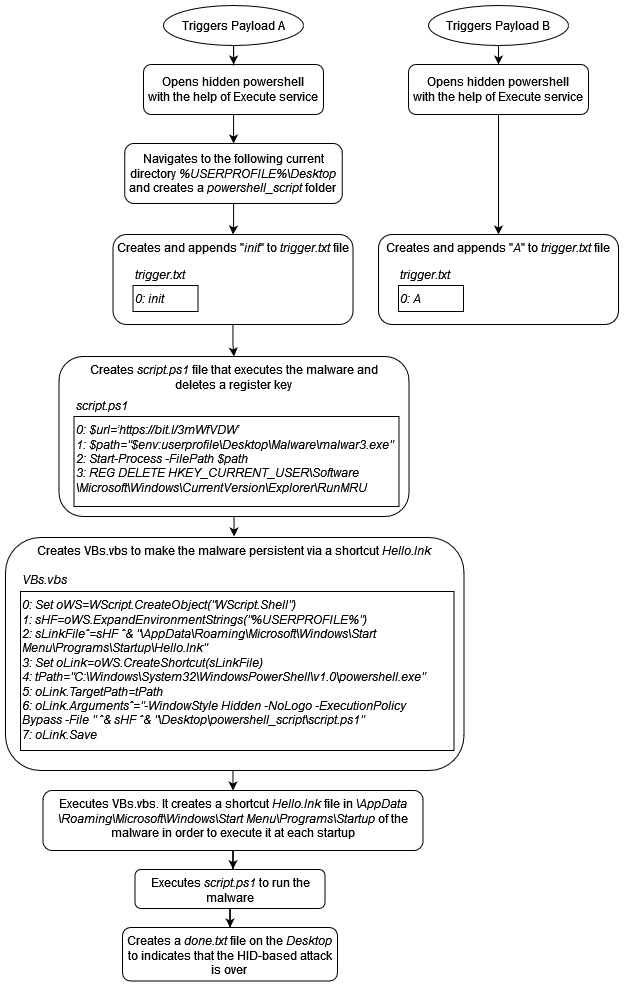
\includegraphics[height=13cm, angle=0, trim={0cm 0cm 0cm 0cm},clip]{figures/logigramme.png}
    \caption{HID-device's flowchart payload.}
    \label{fig:logigram}
\end{figure}

\chapter{Live Demonstration Feedback from the Participants}
\label{annex:feedback}

\begin{itemize}
    \item « The cyberattack of the polar crane was extremely well realised because it was very assiduous and very practical: we directly observe how a human-origin mistake (USB cable plug-in) could have consequences on a NPP site. »
    \item « Cybersecurity workshop was interesting and playful. »
    \item « Cybersecurity workshop was very interesting. Congrats to the job done for preparing it, it was immersive and great. »
    \item « Cybersecurity, very good in form and content, it's an eye-opener on the importance of ensuring safety. »
    \item « Cybersecurity: Discovering new dangers for nuclear facilities. Complexity of protecting against this type of risk, given the development of new technologies (AI in particular). »
    \item « Cyber-crime: Excellent! A return to childhood via the lego sketch, which can be moved and even controlled by the PLC. The workshop on cyber-security really made us realize that evil can lurk anywhere... very instructive! »
    \item « Polar crane hacking: very good, very entertaining, with visual elements. The trainee presented extremely well (very good popularization for non-experts), [...]. I'd perhaps recommend a longer workshop (to allow more questions) and with fewer people, to allow people to move around the polar crane demo and the engineering workstation. »
\end{itemize}


% %%%%%%%%%%%%%%%%%%%%%%%%%%%%%%%%%%%%%%
%
% In case you ever need an (optional) appendix.
%
% You need the following items:
% \begin{itemize}
% \item A box
% \item Crayons
% \item A self-aware 5-year old
% \end{itemize}